\section{Problem Statement}
\lipsum[7-8] 

For single resource reference use: 
\begin{quote}
    \begin{verbatim}
        \cite{das2022boosting}
    \end{verbatim}
\end{quote}

For example, The authors \cite{das2022boosting} claimed that boosted guided ensemble technique can enhance the results of machine learning models.

For multiple resources reference use: 
\begin{quote}
    \begin{verbatim}
        \cite{das2022boosting, sharmin2022invest}
    \end{verbatim}
\end{quote}

For example, The authors \cite{das2022boosting, sharmin2022investigation, uddin2022multi} claimed that boosted guided ensemble technique can enhance the results of machine learning models. 

\section{Motivation}
\lipsum[4-5]

\section{Contributions}
\lipsum[4-5]

\section{Poster Presentation}
\lipsum[1-1]
An overview of the poster presentation is shown in Fig.~\ref{fig:poster_presentation}.

\begin{figure}[H]
\centering
  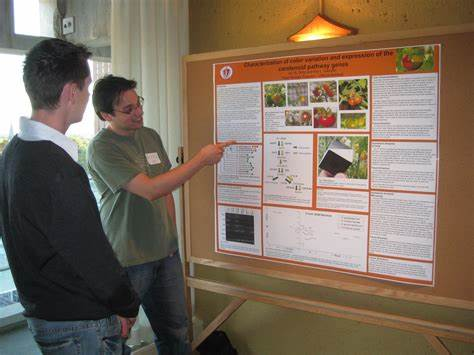
\includegraphics[width=\linewidth]{figures/poster.jpg}
  \caption{Example of poster presentation.}
  \label{fig:poster_presentation}
\end{figure}

\subsection{Subsection of Test}
\lipsum[1-2]
\subsection{Subsection 2 of Test}
\lipsum[1-2]

\section{Report Outline}
In this section, you have to outline the chapters of this report by referencing those. 

\lipsum[1-1]